% Interim Report in CVPR 2024 style
% Note: Compile this file with the official CVPR template files (cvpr.sty).
\documentclass[10pt,twocolumn,letterpaper]{article}
\newif\ifcvprtemplate
\IfFileExists{cvpr.sty}{\cvprtemplatetrue}{\cvprtemplatefalse}
\ifcvprtemplate
\usepackage[review]{cvpr}
\else
\usepackage[margin=1in]{geometry}
\usepackage[numbers,sort&compress]{natbib}
\fi
\usepackage{times}
\usepackage{epsfig}
\usepackage{graphicx}
\usepackage{amsmath}
\usepackage{amssymb}
\usepackage{microtype}
\usepackage{booktabs}
\usepackage{multirow}
\usepackage{array}
\usepackage{tabularx}
\usepackage{enumitem}
\usepackage{url}
\usepackage{tikz}
\usetikzlibrary{positioning,arrows.meta,shapes.geometric}

\newcolumntype{Y}{>{\raggedright\arraybackslash}X}

% Improve paragraph justification in narrow two-column layout.
\setlength{\emergencystretch}{2em}

\def\cvprPaperID{0000}
\def\confName{CVPR}
\def\confYear{2024}

\begin{document}

\title{VokVision: Interim Project Report\\
Monocular Multi-view 3D Reconstruction for Mobile Users}

\author{Team Name Omitted for Blind Review}
\maketitle

\begin{abstract}
This interim report presents the current status of \textbf{VokVision}, a mobile-first computer vision system for 3D scene reconstruction from user-captured multi-view RGB images. The current branch (\textit{SAM\_implementation}) supports upload, asynchronous job orchestration, MASt3R-based mapping, and Gaussian Splatting training interfaces. We summarize problem scope, user interface progress, related work, dataset and metric choices, preliminary system analysis, compute requirements, individual ownership, and next milestones.
\end{abstract}

\section{Problem Statement}
\textbf{Goal.} Build an application where a user captures a short burst of photos of an object or small scene on a phone and obtains a downloadable 3D representation.

\textbf{Input.} The current system accepts a set of monocular RGB images (JPEG/PNG) captured from multiple viewpoints. In the present repository snapshot, our test corpus contains 21 JPEG images.

\textbf{Output.} The intended output is a reconstructed 3D artifact (point cloud / Gaussian representation), delivered as \texttt{point\_cloud.ply} through a backend download endpoint.

\textbf{Primary users.} Content creators, students, and prototyping teams who need a simple ``capture-to-3D'' workflow without specialized sensors.

\textbf{System interface.} Users interact through a Flutter mobile app for capture/upload and polling, while a FastAPI backend executes reconstruction asynchronously.

\textbf{Current scope constraints.}
\begin{itemize}[leftmargin=*]
    \item Monocular image-only pipeline (no IMU/LiDAR fusion yet).
    \item Reconstruction quality depends strongly on viewpoint coverage and image quality.
    \item The branch currently does not expose an active SAM segmentation stage in production flow.
\end{itemize}

\section{User Interface and Progress}
\subsection{Interface design}
The UI follows a feature-modular Flutter architecture with dedicated modules for authentication, capture, reconstruction, gallery, and editor flows. The backend exposes REST endpoints: root health, upload, status, and download.

\begin{figure}[t]
\centering
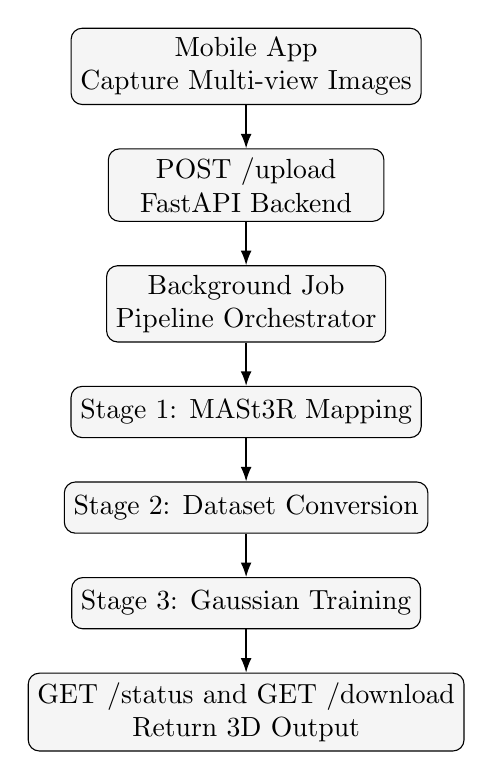
\begin{tikzpicture}[
node distance=0.55cm and 0.35cm,
box/.style={draw, rounded corners, align=center, minimum width=3.5cm, minimum height=0.65cm, fill=gray!8},
arr/.style={-Latex, line width=0.5pt}
]
\node[box] (u1) {Mobile App\\Capture Multi-view Images};
\node[box, below=of u1] (u2) {POST /upload\\FastAPI Backend};
\node[box, below=of u2] (u3) {Background Job\\Pipeline Orchestrator};
\node[box, below=of u3] (u4) {Stage 1: MASt3R Mapping};
\node[box, below=of u4] (u5) {Stage 2: Dataset Conversion};
\node[box, below=of u5] (u6) {Stage 3: Gaussian Training};
\node[box, below=of u6] (u7) {GET /status and GET /download\\Return 3D Output};
\draw[arr] (u1) -- (u2);
\draw[arr] (u2) -- (u3);
\draw[arr] (u3) -- (u4);
\draw[arr] (u4) -- (u5);
\draw[arr] (u5) -- (u6);
\draw[arr] (u6) -- (u7);
\end{tikzpicture}
\caption{Current end-to-end system design and UI-driven backend workflow.}
\label{fig:block}
\end{figure}

\subsection{Progress status}

\textbf{Completed components}
\begin{itemize}[leftmargin=*]
    \item Flutter module scaffolding for capture/reconstruction workflow.
    \item FastAPI upload/status/download API endpoints.
    \item Background orchestration shell for 3-stage pipeline.
    \item MASt3R and Gaussian-Splatting repositories integrated in workspace.
\end{itemize}

\textbf{Incomplete / in-progress components}
\begin{itemize}[leftmargin=*]
    \item Stage-2 conversion integration mismatch (script contract issue).
    \item End-to-end success telemetry and error-state reporting.
    \item Active SAM segmentation stage in deployed branch flow.
\end{itemize}

\section{Related Work}
\textbf{MASt3R / DUSt3R family.} DUSt3R and MASt3R reformulate image matching and geometry estimation directly in 3D, reducing brittle feature engineering and improving reconstruction robustness in many unconstrained scenes~\cite{dust3r,mast3r}.

\textbf{COLMAP-style SfM baselines.} Classical SfM systems such as COLMAP remain strong geometry baselines for sparse reconstruction and pose estimation~\cite{colmap}.

\textbf{Neural rendering baselines.} 3D Gaussian Splatting (3DGS) enables real-time rendering while maintaining high fidelity, making it practical for interactive applications compared to slower NeRF-style rendering~\cite{3dgs,nerf}.

\textbf{Segmentation-oriented methods.} Segment Anything (SAM) provides promptable segmentation useful for foreground isolation and object-aware reconstruction filtering~\cite{sam}. This is part of our intended branch roadmap.

\textbf{Chosen baselines for comparison.}
\begin{itemize}[leftmargin=*]
    \item Classical SfM pipeline: COLMAP~\cite{colmap}
    \item Neural rendering: NeRF~\cite{nerf}
    \item Real-time reconstruction target: 3DGS~\cite{3dgs}
\end{itemize}

\section{Datasets and Evaluation Metrics}
\subsection{Dataset snapshot and EDA}
Current internal dataset snapshot used for development testing:
\begin{itemize}[leftmargin=*]
    \item Upload corpus: 22 JPEG images in the latest successful local run.
    \item Reconstruction workspace assets: image and sparse geometry folders available (\texttt{gs\_dataset/images}, \texttt{gs\_dataset/sparse}).
\end{itemize}

\begin{table}[t]
\centering
\caption{Current development dataset snapshot from repository workspace.}
\label{tab:eda}
\begin{tabularx}{\columnwidth}{@{}l c Y@{}}
\toprule
Asset & Count & Notes \\
\midrule
Uploaded images (JPEG) & 22 & Latest local run batch \\
\texttt{gs\_dataset/images} files & 22 & Candidate training views \\
\texttt{gs\_dataset/sparse} files & 5 & Sparse geometry metadata \\
\bottomrule
\end{tabularx}
\end{table}

\textbf{Observed data peculiarities.}
\begin{itemize}[leftmargin=*]
    \item Small-scale internal dataset; not yet diverse across scenes/devices.
    \item Potential viewpoint imbalance (insufficient full 360 coverage).
    \item Real-world blur/exposure variation expected from handheld capture.
\end{itemize}

\subsection{Evaluation metrics}
Module-wise metrics selected for final evaluation:
\begin{itemize}[leftmargin=*]
    \item \textbf{Reconstruction quality:} PSNR, SSIM, LPIPS (rendered view vs. held-out images).
    \item \textbf{Geometry quality:} Chamfer distance / point-cloud completeness where GT exists.
    \item \textbf{System metrics:} end-to-end runtime, GPU memory, CPU RAM, storage footprint.
    \item \textbf{Product metrics:} successful job rate, average time-to-result, API error rate.
\end{itemize}

\textbf{Resource relevance.} The application is compute-heavy at training stage; GPU VRAM and storage throughput dominate runtime.

\section{Analysis of Results (Interim)}
At this checkpoint, we report module-level status using the latest successful local execution (\texttt{run\_local.py --iterations 2500}) on a 22-image project. The pipeline reached end-to-end completion and produced a final \texttt{model.ply} artifact.

\textbf{Latest run highlights (local, CUDA):}
\begin{itemize}[leftmargin=*]
    \item MASt3R reconstruction completed with 2,181,208 points written (conf\(\ge\)1.5).
    \item Object isolation completed with automatic fallback (multi-scale GrabCut+HSV) when SAM2 module was unavailable.
    \item Multi-cue isolation kept 355,770 points at threshold 0.65 and 317,197 points at threshold 0.70; final cleaned object cloud: 8,294 points.
    \item OpenSplat completed 2,500 training steps and wrote \texttt{model.ply} (934.2 KB) and \texttt{cameras.json}.
\end{itemize}

\begin{table}[t]
\centering
\caption{Interim module-wise performance and status (latest local run).}
\label{tab:interim}
\small
\begin{tabularx}{\columnwidth}{@{}l Y Y@{}}
\toprule
Module & Current result & Key metric/status \\
\midrule
Local job orchestration & Functional & 22 images, 2500 iterations \\
MASt3R Stage & Completed & 2,181,208 points written \\
Object isolation stage & Completed & Final cleaned cloud: 8,294 points \\
OpenSplat training & Completed & 2,500 steps, final model written \\
Output artifact & Generated & \texttt{model.ply} (934.2 KB) \\
\bottomrule
\end{tabularx}
\end{table}

\textbf{Observed warnings and operational gaps:}
\begin{itemize}[leftmargin=*]
    \item VLM path was skipped because \texttt{GEMINI\_API\_KEY} was not set.
    \item SAM2 module was unavailable in environment; fallback segmentation was used.
    \item HF Hub requests were unauthenticated (no \texttt{HF\_TOKEN}), with potential rate-limit/performance impact.
    \item Environment health warnings: Python 3.10 support horizon and deprecated \texttt{google.generativeai} package usage.
    \item MASt3R warning indicated missing CUDA-compiled RoPE2D extension (slow PyTorch fallback).
\end{itemize}

\textbf{Bandwidth and storage considerations.} Multi-image uploads are manageable on Wi-Fi, but model artifacts can grow quickly; storage lifecycle policies are needed before scale-out.

\section{Compute Requirements}
\textbf{Current estimate.}
\begin{itemize}[leftmargin=*]
    \item GPU: NVIDIA CUDA-capable GPU (preferably at least 12GB VRAM; higher is preferred for stability).
    \item CPU RAM: 16--32GB recommended for preprocessing and parallel services.
    \item Storage: Fast SSD required for image I/O and output artifacts.
\end{itemize}

\textbf{Can we manage current compute requirements?} For prototype-scale experiments, yes. For sustained team workloads and repeated training runs, we need either queue-based job scheduling on shared GPU servers or cloud GPU instances.

\textbf{Adjustments needed.}
\begin{itemize}[leftmargin=*]
    \item Implement resource-aware scheduling (avoid concurrent heavy jobs on one GPU).
    \item Add output retention/cleanup policy to control storage growth.
    \item Add fallback execution profiles (reduced image resolution / fewer iterations).
    \item Migrate from \texttt{google.generativeai} to \texttt{google.genai} and standardize Python 3.11+ runtime.
    \item Add environment preflight checks for keys/modules (GEMINI\_API\_KEY, HF\_TOKEN, SAM2 availability).
\end{itemize}

\section{Next Steps}
\begin{enumerate}[leftmargin=*]
    \item Promote the successful local path into API-triggered production workflow with identical configs (Owner: Member C, Member B).
    \item Add explicit job states (queued, running, failed, succeeded) and error payload API (Owner: Member B).
    \item Establish reproducible benchmark sheet (PSNR/SSIM/LPIPS, runtime, memory) across multiple scenes (Owner: Member D).
    \item Expand dataset diversity and perform controlled EDA (Owner: Member A, Member D).
    \item Integrate SAM2 path where available and compare against current GrabCut+HSV fallback baseline (Owner: Member C, Member D).
    \item Harden environment/dependency setup (keys, tokens, package/runtime versions) via preflight script (Owner: Member B).
\end{enumerate}

\paragraph{Risk to timeline.}
The highest risk has shifted from stage integration to environment consistency (API keys, optional modules, package/runtime versions). Mitigation is a strict preflight check and reproducible environment manifest.

{\small
\ifcvprtemplate
\bibliographystyle{ieeenat_fullname}
\else
\bibliographystyle{plainnat}
\fi
\bibliography{interim_report_refs}
}

\end{document}
